\documentclass{beamer}
\usepackage[british]{babel}

\usepackage{fontspec} 
%\setsansfont{Arimo}
% \usepackage{lsp-makros}
\useoutertheme{lsp}

\usepackage{lsptitle}

\def\two@digits#1{\ifnum#1<10 0\fi\number#1}
\def\mytoday{\two@digits{\number\day}.\two@digits{\number\month}.\number\year}


\usepackage{xspace,multicol}
\newcommand{\latex}{\LaTeX\xspace}
\usepackage{tikz}


\newcounter{lastpagemainpart}
\footnotesep0pt
\renewcommand{\footnoterule}{}
\usefootnotetemplate{
  \noindent
  \insertfootnotemark\insertfootnotetext}

\let\beamerfn=\footnote
\renewcommand{\footnote}[1]{%
\let\oldfnsize=\footnotesize%
\let\footnotesize=\tiny%
\beamerfn<\thebeamerpauses$\to${#1}%
\let\footnotesize=\oldfnsize}


\date{20 June 2022}

\usepackage{eurosym}  
 
\renewcommand{\centerline}[1]{\hfill#1\hfill\hfill\mbox{}}


\title{\mbox{Diamond open access books} at Language Science Press}
\author{Felix Kopecky}

\usepackage{emoji}

\begin{document}
\lspbeamertitle

\section{Introduction}

\frame{
	\begin{block}{\emoji{waving-hand} About your speaker:}
	\begin{itemize}
		\item Joined LSP in 2015, now filling the role of Publication Manager
		\item Also pursues a PhD at KIT in Computational Argumentation Theory and Social Epistemology
	\end{itemize}
	\end{block}
}

\section{Language Science Press}


\frame{
	\centering\bfseries\Large	The publication process at\\Language Science Press
}


\frame{
	\frametitle{Language Science Press}
	\begin{columns}
		\column{6cm}
		\begin{itemize}
			\item scholar-owned, non-profit publisher
			\item 30 series, autonomous in content and publication decisions
			\item 695 expressions of interest
			\item 180 books published since 2014
			\begin{itemize}
				\item monographs \& edited volumes
				\item 30/year
				\item books from 2021 on the right
			\end{itemize}
			\item books ranging 76--1632 pages
			\item 1.5m total downloads
			\begin{itemize}
				\item 75k for most successful title
			\end{itemize}
		\end{itemize}
		\column{4cm}
		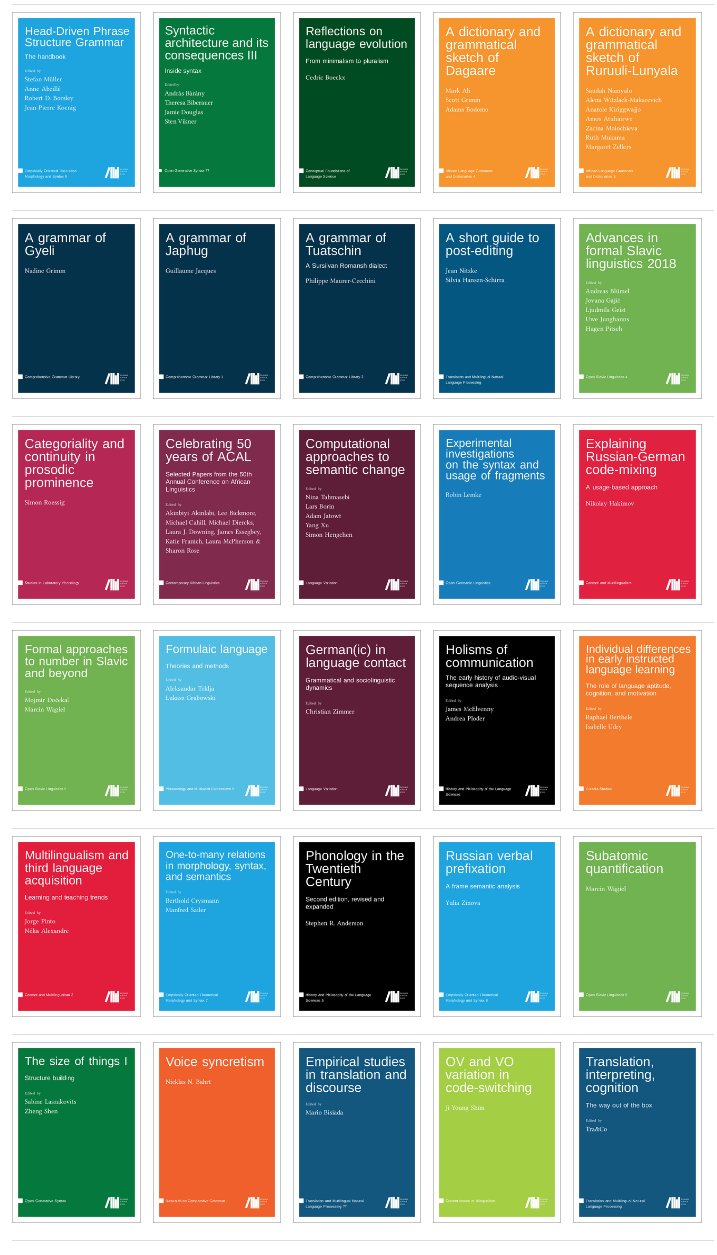
\includegraphics[height=.95\textheight]{output2022.png}
	\end{columns}
}

\frame{\frametitle{LSP publication process}
	\begin{enumerate}
		\item Expressions of interest/submissions can be directed to:
		\begin{itemize}
			\item One of the series directly
			\item The LSP office if uncertain
			\item Proposals for new series to be directed to the Advisory Board
		\end{itemize}
		\item Peer-review on the series editors' terms (open peer review possible)
		\item Community proofreading for style and guidelines
		\item Professional typesetting and layout in cooperation with author/editor, based on \LaTeX
		\item Digital and physical distribution (on demand printing)
	\end{enumerate}
}

{\setbeamertemplate{footline}{}
\frame{\frametitle{Overleaf-integrated workflow}
	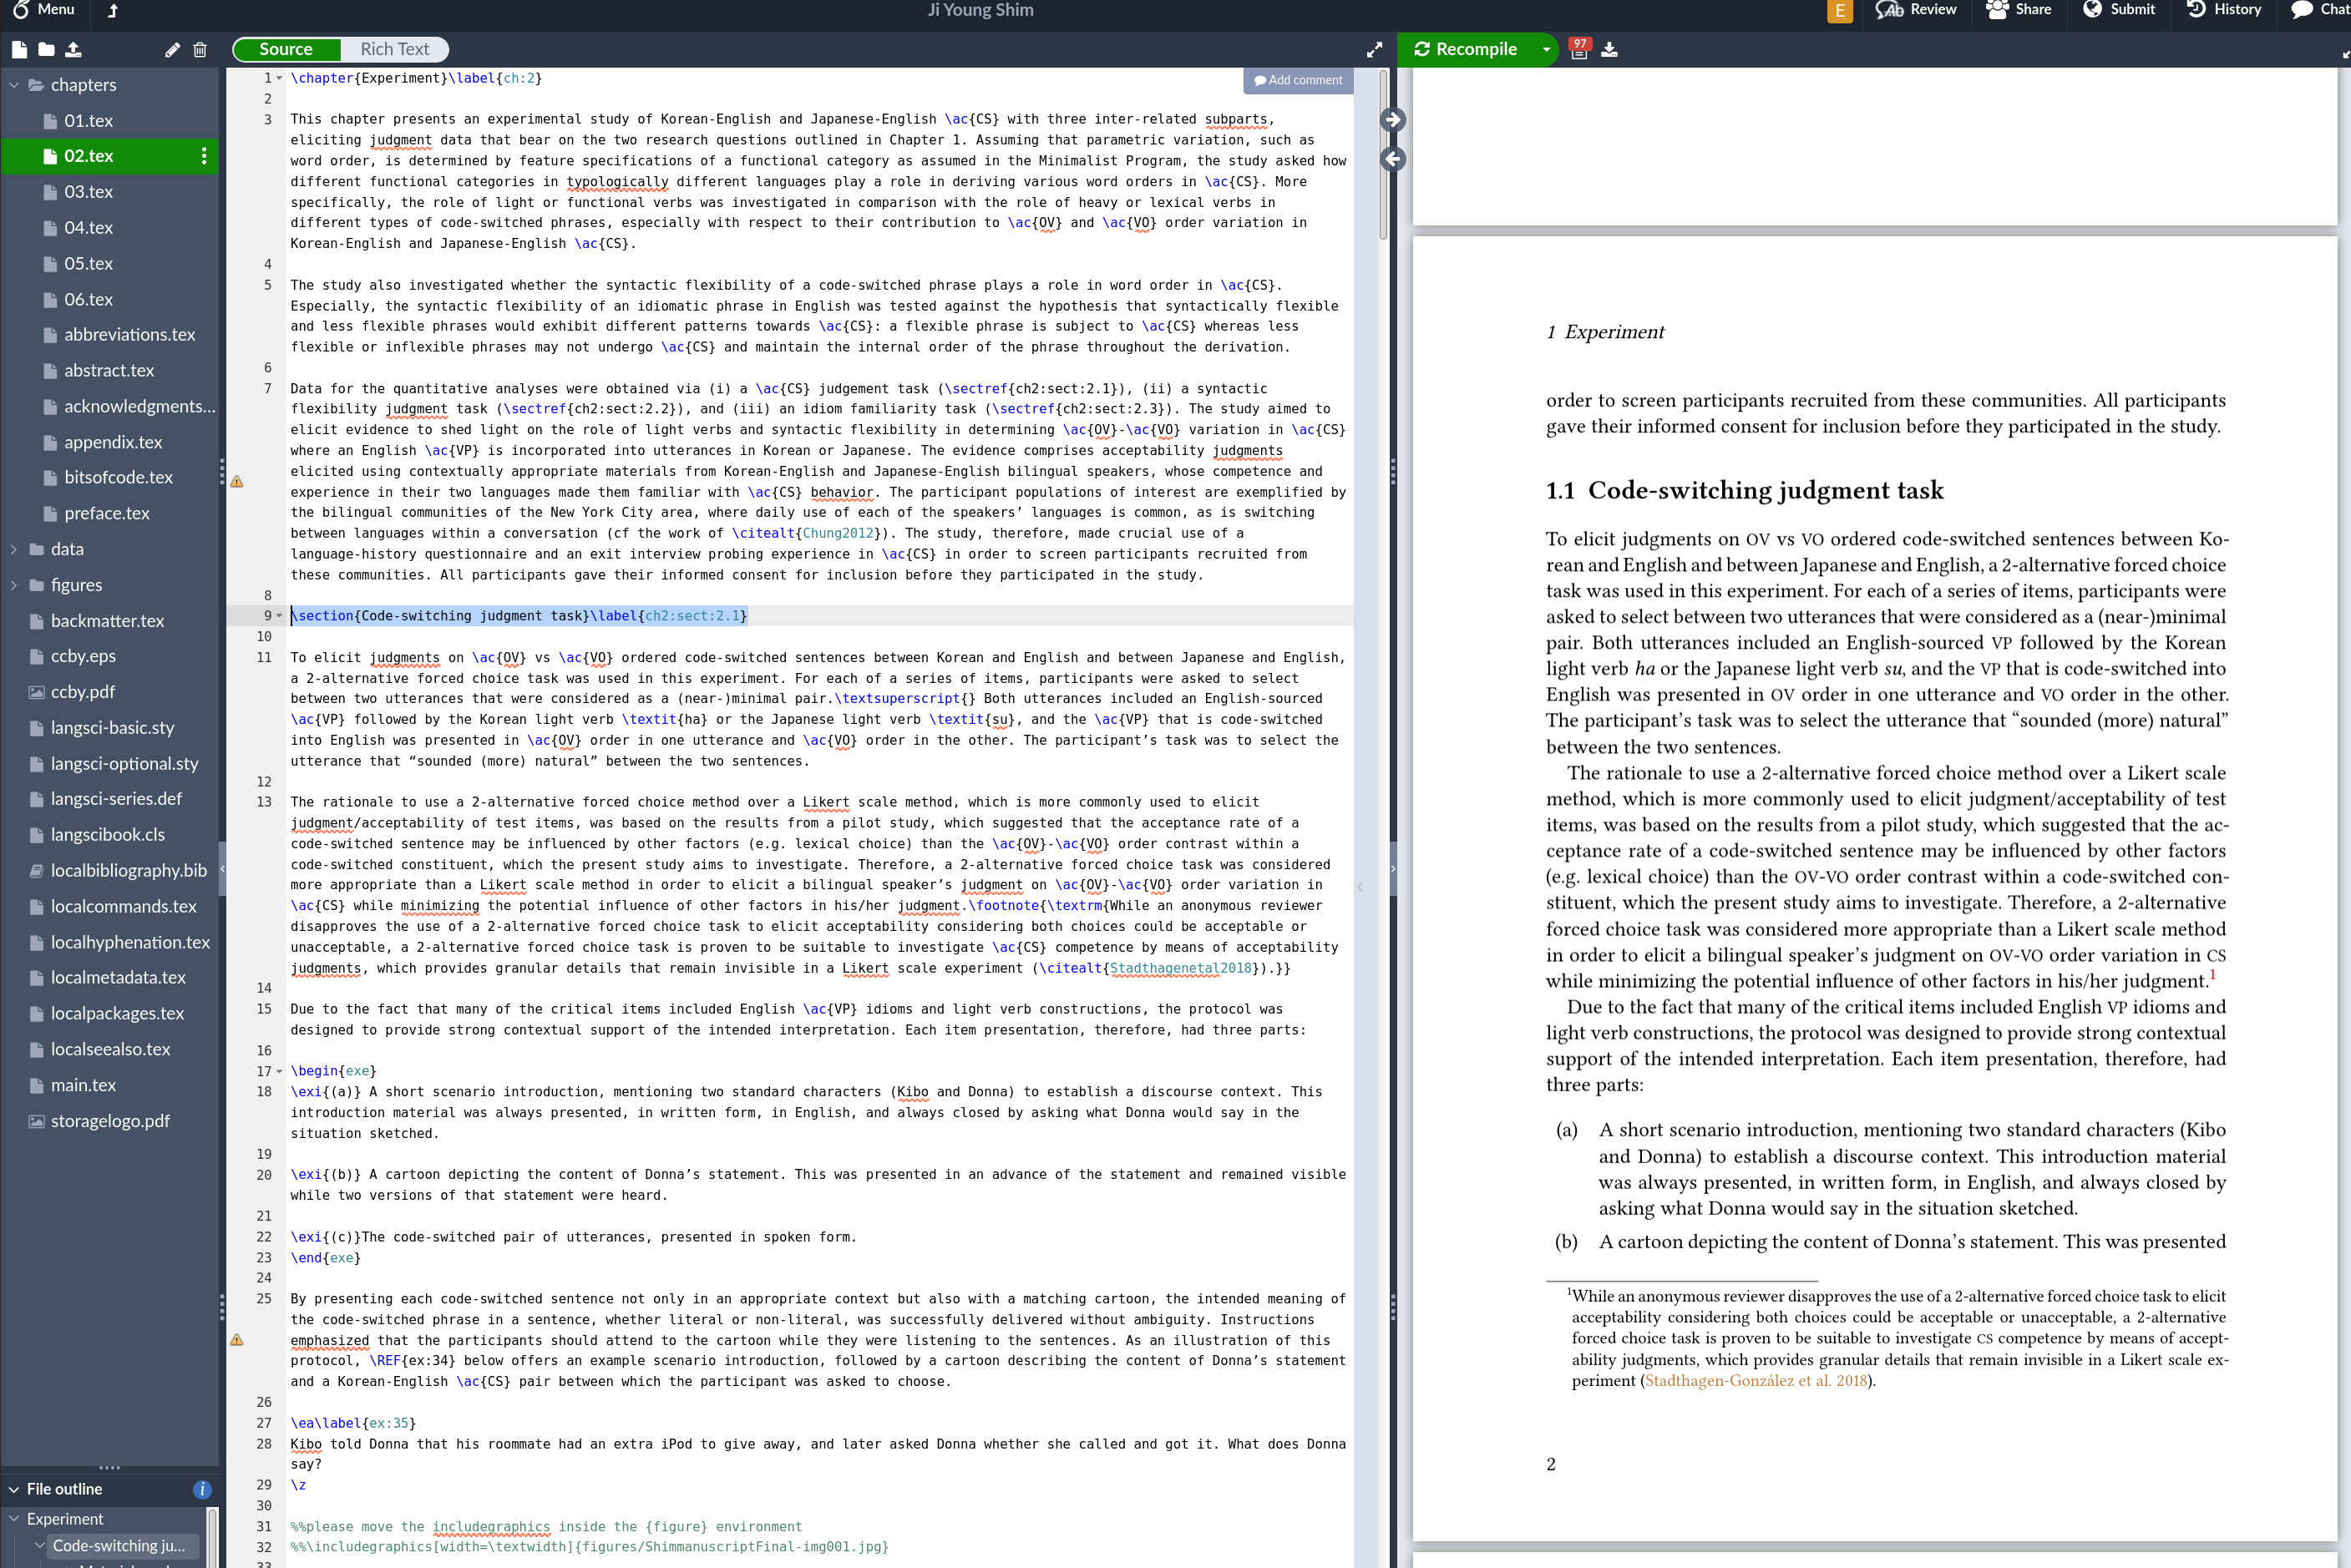
\includegraphics[width=\textwidth]{overleaf.png}
}
}

\section{Open access}

\frame{
	\centering\bfseries\Large	Why publish OA?
}

\frame{\frametitle{Why OA?}
	\begin{block}<+->{Key goals of the OA movement}
		\begin{itemize}
			\item Content be freely available to readers – immediately, and forever
			\item Authors retain copyright
			\item Avoid prohibitive costs of publication
		\end{itemize}
	\end{block}
	
	\begin{block}<+->{Types}
		\begin{itemize}
			\item Green OA			
			\item Gold OA			
			\item Diamond OA
		\end{itemize}
	\end{block}
}

\frame{\frametitle{Types of OA}
	
	\begin{block}{Types}
		\begin{enumerate}
			\item Green OA (self-archiving)
			\begin{itemize}
				\item Business as usual, but:
				\item Authors are allowed to self-archive their work %(e.g. on preprint servers)
				\item Possible restrictions: Embargo periods, not being able to distribute final paper
				\item Not all people agree this is really “open access”.
			\end{itemize}
		\end{enumerate}
	\end{block}
}

\frame{\frametitle{Types of OA}
	
	\begin{block}{Types}
		\begin{enumerate}
			\item[2.] Gold OA
			\begin{itemize}
				\item<1-> Content is freely available to readers, immediately and forever \emoji{thumbsup}
				\item<1-> Author retains copyright \emoji{thumbsup} %trough Creative Commons licenses
				\item<1-> So far, so good, but: Prohibitive costs are common (“APCs”) \emoji{thumbsdown}
				\item[]<1->
				\item<2-> Example:
				\begin{itemize}
					\item KIT library funds APCs: up to €\,2,000
					\item Fees in FK's fav.\ journal for gold OA: €\,2,290 
					\item[] (This is \alert<2>{a lot} of money considering the services offered.)
				\end{itemize} 
%				\item<3-> Example 2: Journal requires €\,20 submission charge for gold OA
%				\item[]<3-> (Example for non-prohibitive costs – sadly, the minority)
			\end{itemize}
		\end{enumerate}
	\end{block}
}

\frame{\frametitle{Types of OA}
	
	\begin{block}{Types}
		\begin{enumerate}
			\item[3.] Diamond OA
			\begin{itemize}
				\item<1-> Content is freely available to readers, immediately and forever \emoji{thumbsup}
				\item<1-> Author retains copyright \emoji{thumbsup}%trough Creative Commons licenses
				\item<1-> No submission or processing costs for authors \emoji{thumbsup}
			\end{itemize}
		\end{enumerate}
	\end{block}
}

\frame{\frametitle{Who pays for diamond OA?}
\begin{block}{The consortial model}
	Costs are covered by third parties, such as consortia of academic institutions\pause 
	\begin{itemize}
		\item Language Science Press is funded by 115 institutions world wide (thank you to the library of Goethe-Universität!)
		\item The funding is organised by Knowledge Unlatched, a service provider specialising in consortial funding models
		\item Some independent journals do this on a smaller scale (e.g. sponsor institutions pay €\,100–200 p.a.)
		\item This model proves to be \alert{much more cost-effective} compared to many gold OA models
	\end{itemize}
\end{block}
}


\frame{\frametitle{Diamond OA benefits}
\begin{itemize}
	\item[\emoji{copyright}] You retain the rights to your work %in terms of a Creative Commons license
%	\begin{itemize}
		\item[\emoji{recycle}] Enables re-usage of content 
%	\end{itemize}
	\item[\emoji{telescope}] Scientific merit decides what is published (not financial resources)  %(everyone can publish everything that meets merit)
	\item[\emoji{earth-africa}] Immediately available to everyone who is interested%(everyone can read everything)
	\item[\emoji{infinity}] Long-term, wide circulation of your work 
	\item Perfect fit for an open science approach (open data, open source, open peer review)
\end{itemize}}

%\setcounter{framenumber}{\thelastpagemainpart}
\end{document}
